
\section{Intro a 3D}


% https://www.mathematik.uni-marburg.de/~thormae/lectures/graphics1/graphics_4_1_eng_web.html#1
\frame{
\frametitle{OpenGL}
\begin{itemize}
\item OpenGL significa Open Graphics Library, un estándar para la progamación de gráfica.
\item Los comandos de gráficos son implementados por el controlador de la tarjeta gráfica y, por lo tanto, son independientes del hardware de la tarjeta gráfica, del sistema operativo y del administrador de ventanas empleado.
\item Los comandos de gráficos están razonablemente cercanos al hardware y son suficientes para lograr la funcionalidad principal
\item Varias bibliotecas y frameworks se basan en OpenGL y permiten la programación a un mayor nivel de abstracción.
\end{itemize}
}

\frame{
\frametitle{OpenGL Versions}
\begin{itemize}
\item Desde su introducción (1992) OpenGL se ha ampliado continuamente para admitir nuevas funciones de tarjetas gráficas.
\item OpenGL 1.0 (1992), OpenGL 1.1 (1997), OpenGL 1.2 (1998), OpenGL 1.3 (2001), OpenGL 1.4 (2002), OpenGL 1.5 (2003)
\item OpenGL 2.0 (2004), OpenGL 2.1 (2006)
\item OpenGL 3.0 (2008), OpenGL 3.1 (2009), OpenGL 3.2 (2009), OpenGL 3.3 (2010)
\item OpenGL 4.0 (2010), OpenGL 4.1 (2010), OpenGL 4.2 (2011), OpenGL 4.3 (2012), OpenGL 4.4 (2013), OpenGL 4.5 (2014), OpenGL 4.6 (2017)
%\item En esta ponencia, se combina la versi
\item A partir de la  versión 3.1, el Pipeline de funciones fijo ya no esta soportado, por lo cual es necesario implementar shaders, lo cual dificulta el aprendizaje.
\end{itemize}
}


\frame{
\frametitle{OpenGL ES y WebGL}
\begin{itemize}
\item OpenGL ES (Embedded System) es una versión de OpenGL con funcionalidad reducida para teléfonos móviles, televisores, tabletas, etc.
\item OpenGL ES 1.0 (2003): similar a OpenGL 1.3 (Pipeline Fijo)
\item OpenGL ES 1.1 (2004): similar a OpenGL 1.5 (compatible con versiones anteriores)
\item OpenGL ES 2.0 (2007): similar a OpenGL 2.0 (no compatible con versiones anteriores)
\item OpenGL ES 3.0 (2012): similar a OpenGL 3.3 
\item OpenGL ES 3.1 (2014): similar a OpenGL 4.3
\item OpenGL ES 3.2 (2015): similar a OpenGL 4.3
\item OpenGL ES 3.3 (2017): similar a OpenGL 4.6
%\item OpenGL ES se utiliza para la salida de gráficos asistidos por hardware en muchos teléfonos inteligentes (por ejemplo, iPhone de Apple y dispositivos basados en Android)
\item WebGL esta basado en OpenGL ES 2.0 (y WebGL 2.0 en OpenGL ES 3.0) y permite gráficos 3D en páginas web (compatible con la mayoría de navegadores)
\end{itemize}
}


% Aventar aqui el modelo de VonNeumann
%\frame{
%\frametitle{Arquitectura de Von Neumann}
%\begin{columns}
%\begin{column}{0.59\textwidth}
%\begin{itemize}
%\item Fue publicada por primera vez por John von Neumann en 1945.
%\item Su diseño de arquitectura informática consta de una Unidad de Control, Unidad Aritmética y Lógica (ALU), Unidad de Memoria, Registros y Entradas / Salidas.
%\item La arquitectura de Von Neumann se basa en el concepto de computadora de programa almacenado, donde los datos de instrucción y los datos del programa se almacenan en la misma memoria. 
%\end{itemize}
%\end{column}
%\begin{column}{0.39\textwidth}
%\begin{center}
%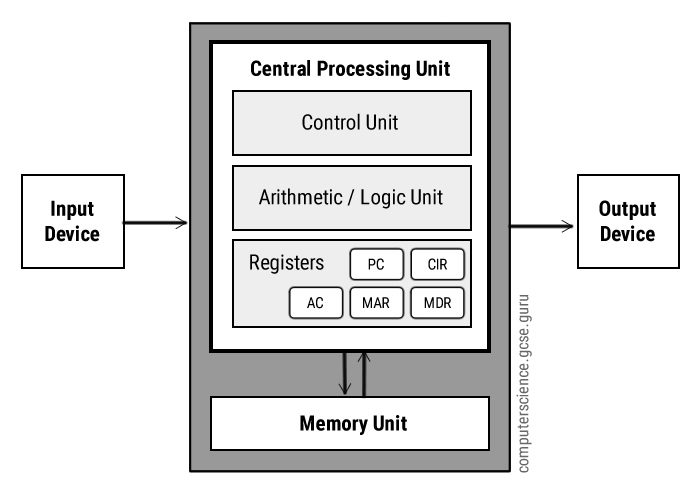
\includegraphics[width=0.9\textwidth]{2022_TallerGraficacion/Figs/Von-Neumann-Architecture-Diagram}\\
%\end{center}
%\begin{block}{Secuencia de operaciones}
%\textbf{En serie.}
%\end{block}
%\end{column}
%\end{columns}
%}



\begin{frame}{Limitaciones del Modelo de Von Neumann}
\begin{columns}
\begin{column}{0.60\textwidth}  
\begin{itemize}
\item La mayoría de las computadoras y teléfonos inteligentes tienen procesadores multicore
\item Un CPU aún cuando es rápido, no esta diseñado para manejar de manera eficiente operaciones de punto flotante. 
\item Un CPU no tiene el suficiente poder de cómputo para generar gráficos en 3D complejos en tiempo real. 
\item Para procesamiento gráficos es necesario el uso de unidades de procesamiento especializadas.
\end{itemize}
\end{column}
\begin{column}{0.40\textwidth}  
    \begin{center}
     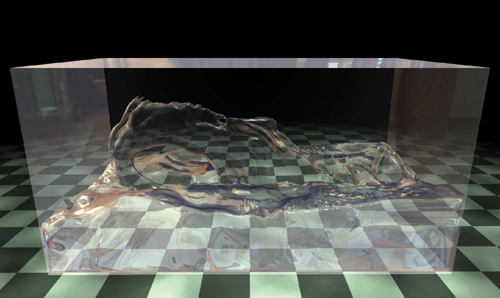
\includegraphics[width=\textwidth]{2022_TallerGraficacion/Figs/Nvidia_Fluido.jpg}\\
          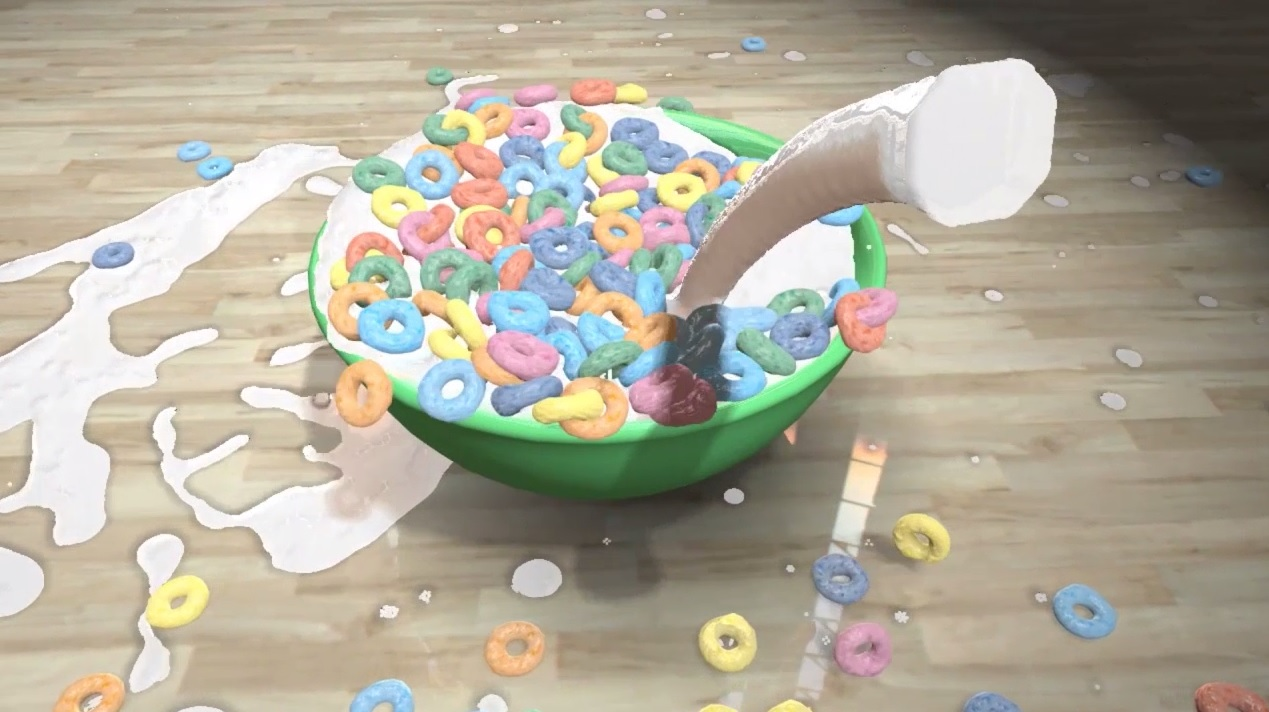
\includegraphics[width=\textwidth]{2022_TallerGraficacion/Figs/Nvidia_FleX_cereal.jpg}\\
     \end{center}
\end{column}
\end{columns}
\end{frame}



\begin{frame}{SoCs para Teléfonos Inteligentes}
\begin{columns}
\begin{column}{0.60\textwidth}  
\begin{itemize}
\item El término SoC significa system-on-a-chip.
\item Un SoC es un sistema completo contenido en un solo circuito integrado.
\item La combinación de todos sus componentes en una sola unidad de procesamiento permite un ahorro de energía significativo. 
\item Bloques comunes en un SoC:
\begin{itemize}
\item Central Processing Unit (CPU).
\item Graphics Processing Unit (GPU).
\item Image Processing Unit (ISP).
\item Digital Signal Processor (DSP).
\item Neural Processing Unit (NPU).
\item Video encoder/decoder.
\item Modems.
\end{itemize}
%\item La mayoría de los teléfonos inteligentes tienen integrado un GPU
%\item Un GPU es una unidad especializada de procesamiento para operaciones de punto flotante en paralelo.
%\item El Samsung S10 Qualcomm Snapdragon 855 SoC (tiene un CPU de 8 núcleos y un GPU dedidado para gráficos (Adreno 640).
\end{itemize}
\end{column}
\begin{column}{0.40\textwidth}  
    \begin{center}
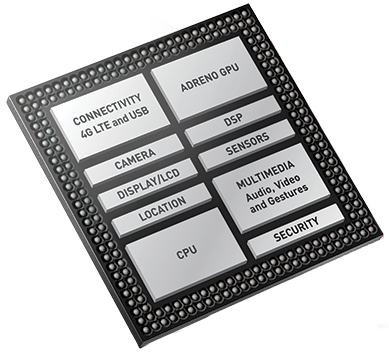
\includegraphics[width=0.65\textwidth]{2022_TallerGraficacion/Figs/qualcomm_snapdragon410_block}\\
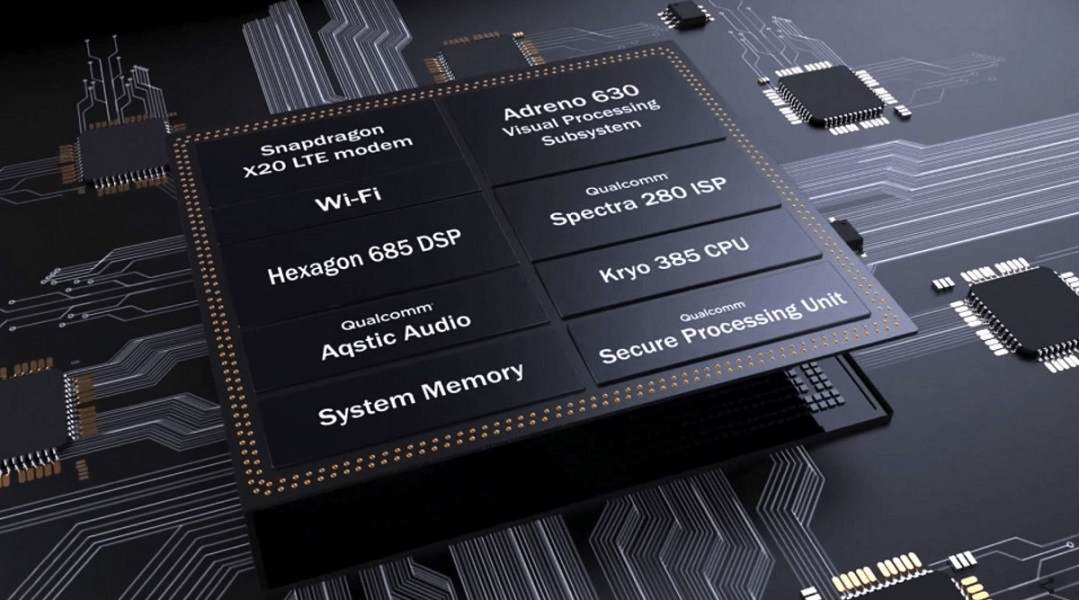
\includegraphics[width=0.85\textwidth]{2022_TallerGraficacion/Figs/Snapdragon-855-1}
     \end{center}
\end{column}
\end{columns}
\end{frame}


%\frame{
%\frametitle{¿Qué es un GPU (Graphics Processing Unit)?}
%\begin{columns}
%\begin{column}{0.49\textwidth}
%\begin{itemize}
%\item Un GPU es un procesador formado por muchos núcleos más pequeños y especializados, especializada en operaciones de punto flotante en paralelo.
%\item Al trabajar conjuntamente, los núcleos ofrecen un desempeño masivo cuando se puede dividir una tarea de procesamiento y es procesada por muchos núcleos.
%\item Por ejemplo, el Samsung S10 utiliza un Qualcomm Snapdragon 855 SoC (tiene un CPU de 8 núcleos y un GPU dedidado para gráficos (Adreno 640).
%\end{itemize}
%\end{column}
%\begin{column}{0.19\textwidth}
%\begin{center}
%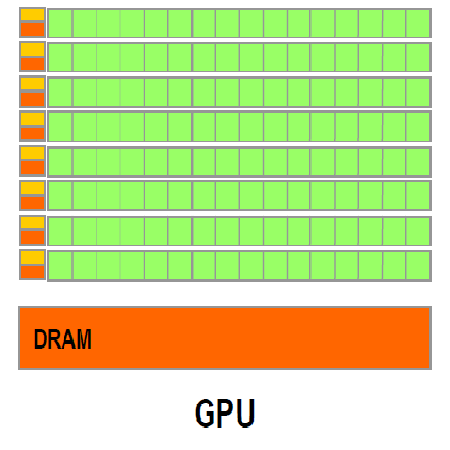
\includegraphics[width=0.9\textwidth]{2022_TallerGraficacion/Figs/GPU}\\
%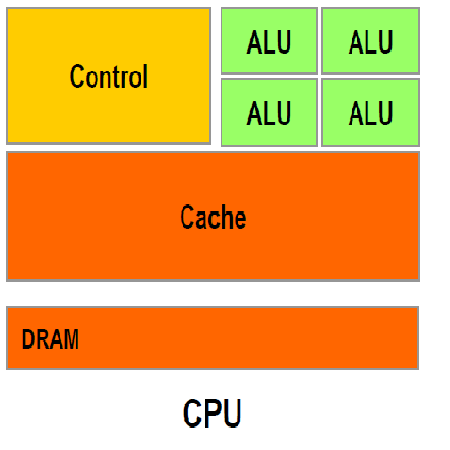
\includegraphics[width=0.9\textwidth]{2022_TallerGraficacion/Figs/CPU}\\
%\end{center}
%\end{column}
%\begin{column}{0.30\textwidth}  
%    \begin{center}
%     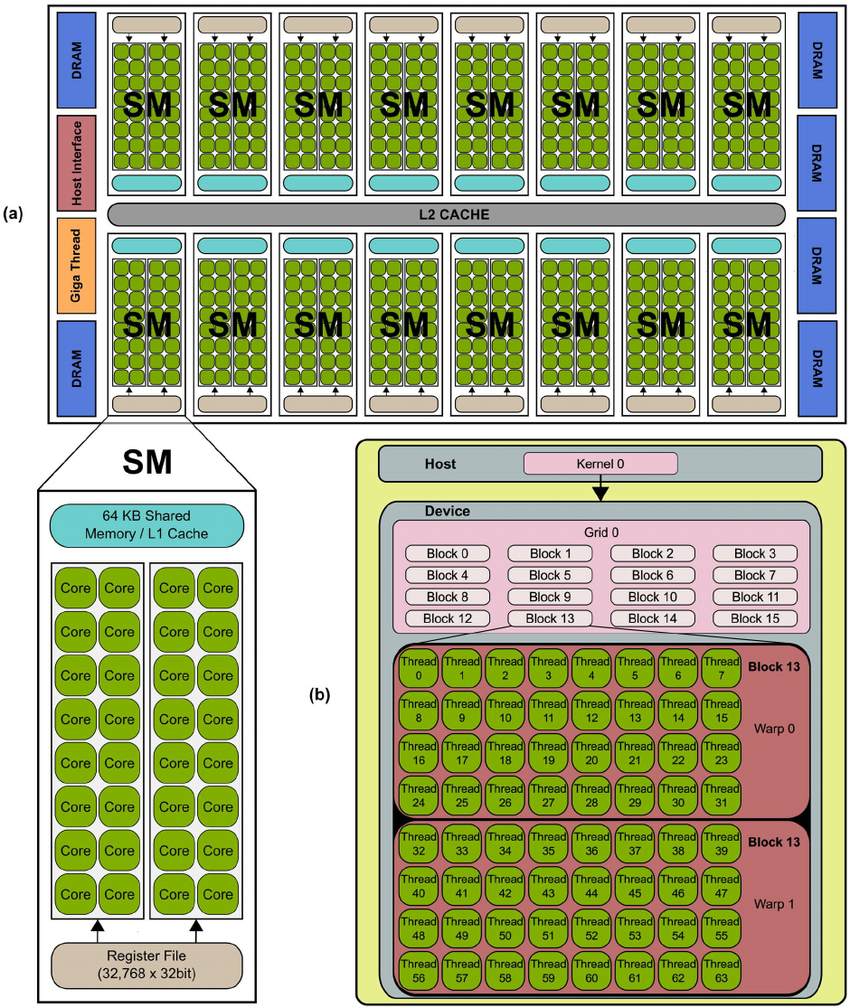
\includegraphics[width=\textwidth]{2022_TallerGraficacion/Figs/Typical-NVIDIA-GPU-architecture}
%     \end{center}
%\end{column}
%\end{columns}
%}

%\begin{frame}{GPU}
%\begin{columns}
%\begin{column}{0.70\textwidth}  
%\begin{itemize}
%%\item La mayoría de los teléfonos inteligentes tienen integrado un GPU
%\item Un GPU es una unidad especializada de procesamiento para operaciones de punto flotante en paralelo.
%\item El Samsung S10 Qualcomm Snapdragon 855 SoC (tiene un CPU de 8 núcleos y un GPU dedidado para gráficos (Adreno 640).
%\end{itemize}
%\end{column}
%\begin{column}{0.30\textwidth}  
%    \begin{center}
%     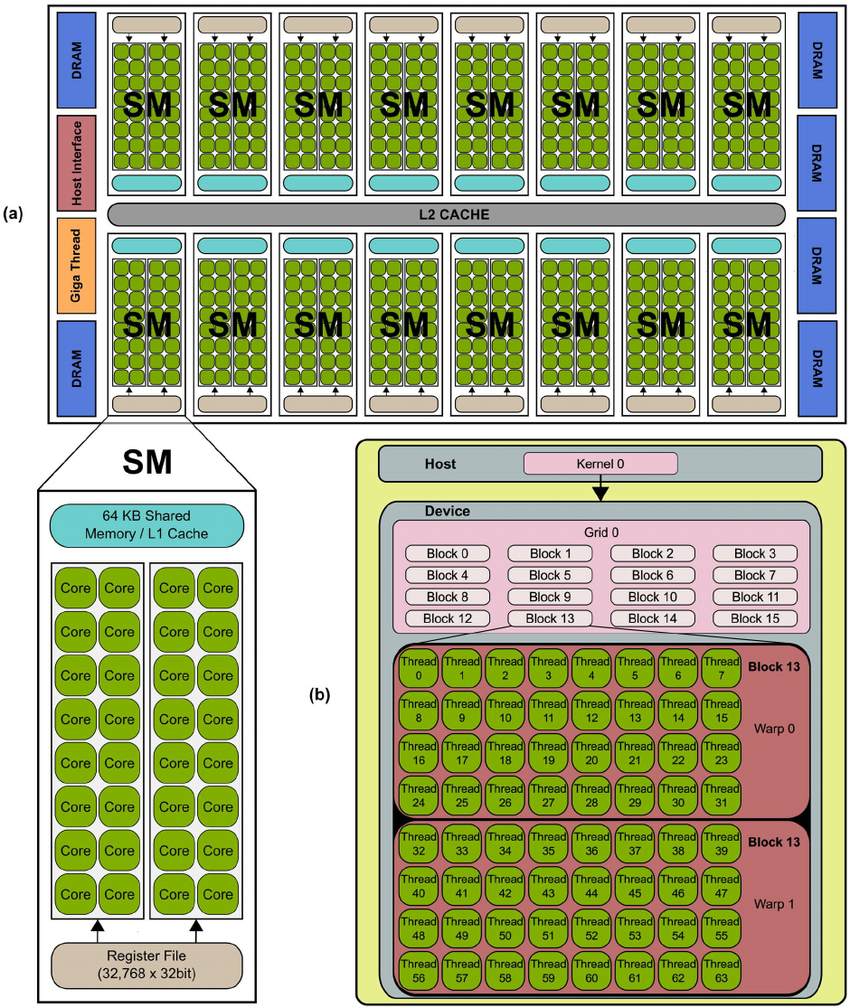
\includegraphics[width=\textwidth]{2022_TallerGraficacion/Figs/Typical-NVIDIA-GPU-architecture}
%     \end{center}
%\end{column}
%\end{columns}
%\end{frame}


%\begin{frame}{CPU-GPU}
%\begin{columns}
%\begin{column}{0.50\textwidth}  
%\begin{itemize}
%\item La mayoría de los teléfonos inteligentes tienen integrado un GPU
%\item Un GPU es una unidad especializada de procesamiento para operaciones de punto flotante en paralelo.
%\item El Samsung S10 Qualcomm Snapdragon 855 SoC (tiene un CPU de 8 núcleos y un GPU dedidado para gráficos (Adreno 640).
%\end{itemize}
%\end{column}
%\begin{column}{0.50\textwidth}  
%    \begin{center}
%     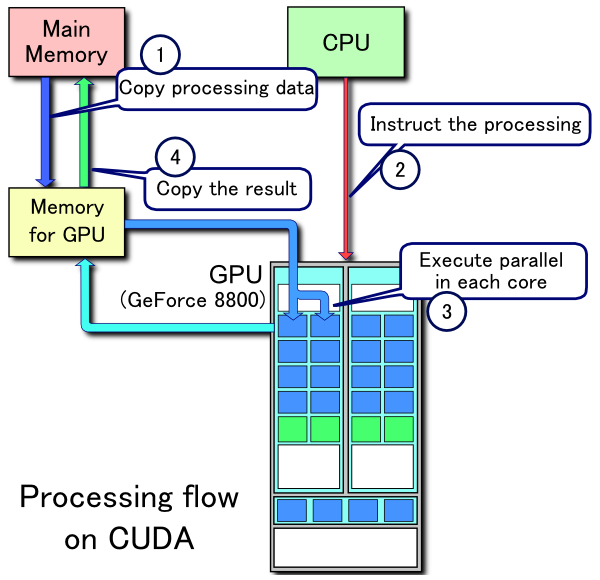
\includegraphics[width=\textwidth]{2022_TallerGraficacion/Figs/CUDA_processing_flow}
%     \end{center}
%\end{column}
%\end{columns}
%\end{frame}





	
\begin{frame}{OpenGL Shading Language}
\begin{itemize}
\item Las aplicaciones móviles son ejecutadas principalmente en el CPU y la memoria principal
\item Para procesamiento de gráficos, los programas son ejecutados en el GPU el cual tiene su propia memoria local (memoria gráfica). Existen dos tipos de procesadores
\begin{itemize}
\item El vertex processor
\item El fragment processor
\end{itemize}
\item Los programas del GPU son escritos en un lenguaje llamado Shading Language (Lenguaje de sombreado). 
\item La mayoría de los GPUs adoptaron el lenguaje de OpenGL shading Language (OGSL)
\end{itemize}
\end{frame}

%\begin{frame}{OpenGL}
%OpenGL signfiica Open Graphics Library, un estándar para la progamación de gráfica.
%El OpenGL Shading Language es un lengauje de alto nivel (cuya sintaxis es parecida a C) diseñado para procesamiento en paralelo en un GPU. 
%\end{frame}



%\begin{frame}{OpenGL Pipeline}
%El GPU tiene dos tipos de procesadores:
%\begin{itemize}
%\item El vertex processor
%\item El fragment processor
%\end{itemize}
%Los programas deben ser cargados en cada procesador.
%\end{frame}

\begin{frame}{OpenGL Pipeline}
    \begin{center}
    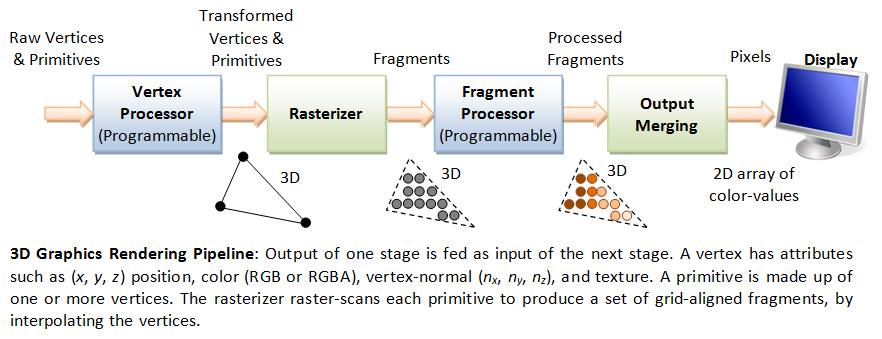
\includegraphics[width=\textwidth]{2022_TallerGraficacion/Figs/Graphics3D_Pipe}
    \end{center}
\end{frame}


\begin{frame}{OpenGL Pipeline (2)}
    \begin{center}
    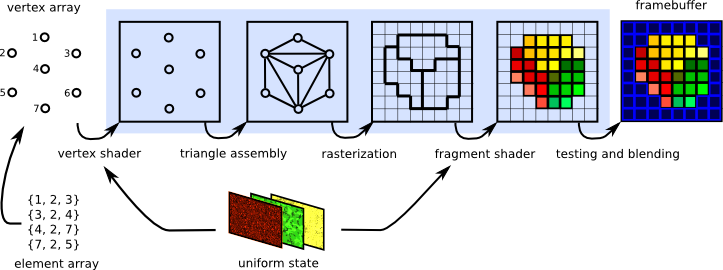
\includegraphics[width=\textwidth]{2022_TallerGraficacion/Figs/evasgl-graphics-pipeline}
    \end{center}
\end{frame}

\begin{frame}{Transformaciones}
    \begin{center}
    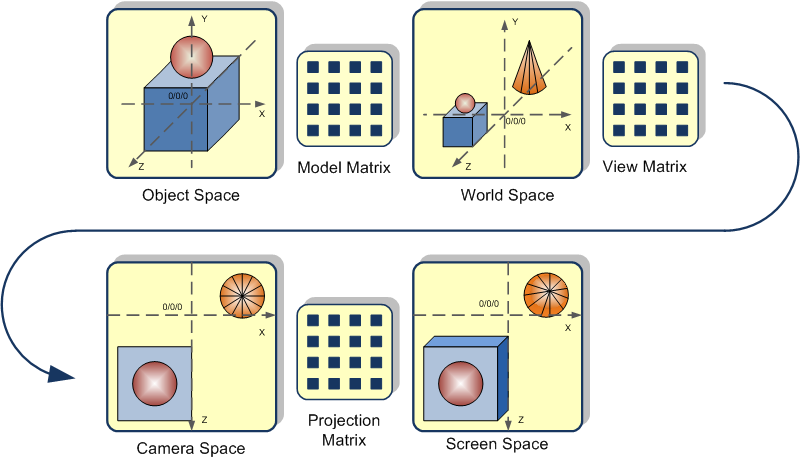
\includegraphics[width=0.75\textwidth]{2022_TallerGraficacion/Figs/ModelViewProjection_MVP_Matrix}
    \end{center}
\end{frame}


%\section{Shading Language}
%\begin{frame}{}
%\end{frame}

%\section{Primitivas 2D}
\begin{frame}{Dibujo de Primitivas}
%\begin{itemize}
%\item Primer Demo del Imperial College (Dibujar un triangulo)
%\item ** Dibujar un Hexagono
%\item ** Explicar primitivas graficas 
%\end{itemize}
%\begin{block}{Demo \#1}
%Dibujar un Triangulo en 2D
%\end{block}
\begin{columns}
\begin{column}{0.4\textwidth}
\begin{itemize}
\item Para dibujar cualquier superficie en OpenGL, se debe triangular los vértices adyacentes para formar polígonos (generalmente triangulos).
\item Se requieren de dos triangulos para dibujar un cuadrado.
\end{itemize}
\begin{block}{Demo \#1}
Dibujar un Triangulo en 2D
\end{block}

\end{column}
\begin{column}{0.3\textwidth}
\begin{center}
 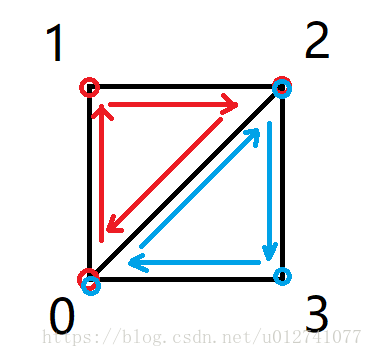
\includegraphics[width=0.98\textwidth]{2022_TallerGraficacion/Figs/Cuadrado_Formado_por_Triangles}
 \end{center}

\end{column}
\begin{column}{0.3\textwidth}
\begin{center}
 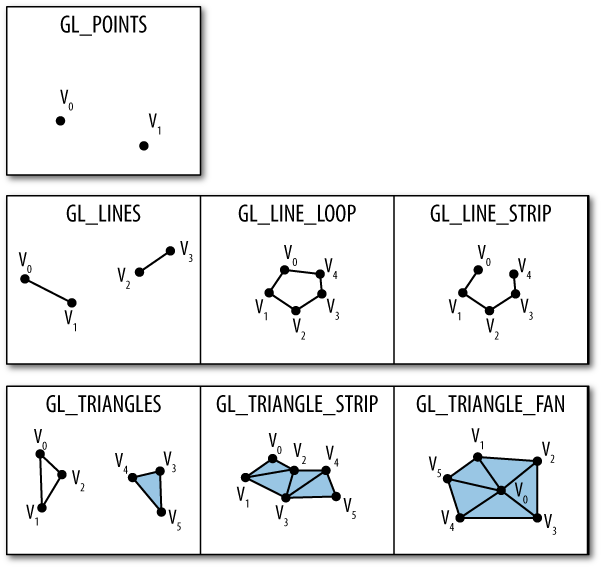
\includegraphics[width=0.98\textwidth]{2022_TallerGraficacion/Figs/PrimitiavasOpenGL}
 \end{center}
\end{column}
\end{columns}


\end{frame}

\begin{frame}{Experimentado con Primitivas}
\begin{columns}
\begin{column}{0.5\textwidth}
\begin{itemize}
\item Es posible dibujar objetos complejos si se tiene un entendimiento correcto de las primitivas 
\item Por ejemplo: Dibujar un Hexagono Relleno/Alambrico. 
\end{itemize}
\end{column}
\begin{column}{0.5\textwidth}
\begin{center}
 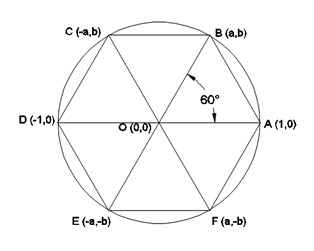
\includegraphics[width=0.98\textwidth]{2022_TallerGraficacion/Figs/Hexagono}
 \end{center}
\end{column}
\end{columns}

\end{frame}







%\section{Primitivas 3D}
\begin{frame}{Cubo 3D}
%\begin{itemize}
%\item Lesson 00, Colored Cube
%\item Letra A
%\item Lesson 01, Transformaciones
%\item Esfera 
%\end{itemize}

\begin{columns}
\begin{column}{0.4\textwidth}



\begin{block}{Demo \#2}
Cubo en OpenGL
\end{block}
\begin{center}
 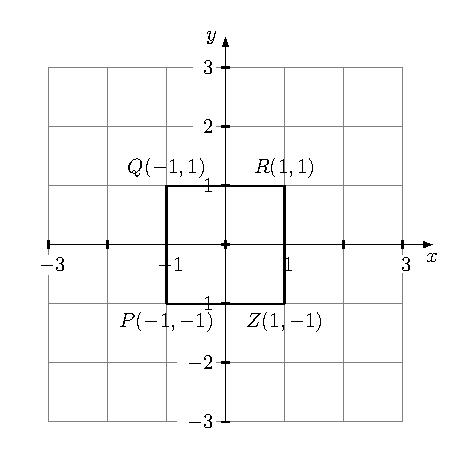
\includegraphics[width=0.98\textwidth]{2022_TallerGraficacion/Figs/planocartersiano}
 \end{center}
\end{column}
\begin{column}{0.4\textwidth}
\begin{center}

  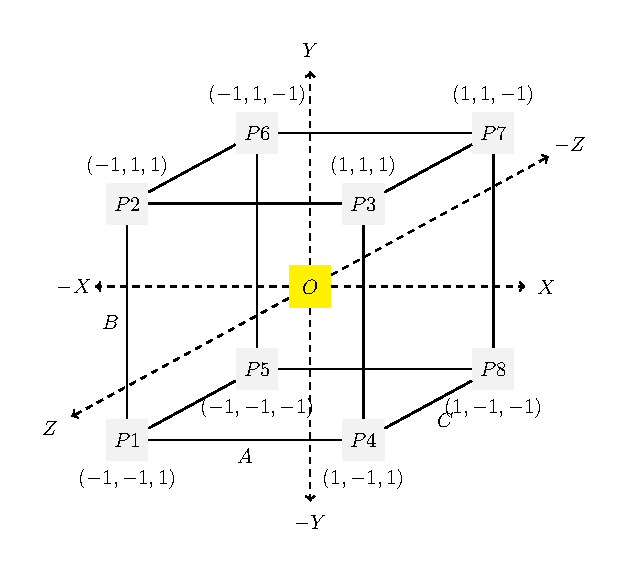
\includegraphics[width=0.98\textwidth]{2022_TallerGraficacion/Figs/cube}
 \end{center}

\end{column}
\begin{column}{0.3\textwidth}
\begin{center}

 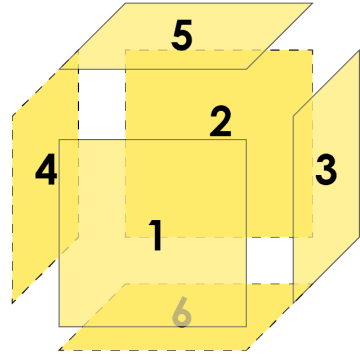
\includegraphics[width=0.98\textwidth]{2022_TallerGraficacion/Figs/CarasCubo}
 \end{center}
\end{column}
\end{columns}

\end{frame}




\begin{frame}{Objetos Complejos en OpenGL}
\begin{itemize}
\item Una vez que se entiende como generar las coordenadas de poligonos y asignarles un color, es posible construir objetos 3D complejos.
\end{itemize}

\begin{block}{Demo \#3}
Objetos Complejos en OpenGL (Letra A)
\end{block}
\end{frame}


\begin{frame}{Transformaciones}
\begin{columns}
\begin{column}{0.5\textwidth}
\begin{itemize}
\item \textbf{Translación.} Es un cambio en la posición de los objetos en cualquiera de los ejes.
\item \textbf{Escalamiento.} Es un cambio en el tamaño de un objeto con respecto a sus dimensiones en cualquiera de los ejes. 
\item \textbf{Rotación.} La orientación de un objeto puede ser cambiada mediante un ángulo de rotación.

\end{itemize}
\begin{block}{Demo \#4}
Transformaciones y Animación en OpenGL
\end{block}
\end{column}
\begin{column}{0.5\textwidth}
\begin{center}
% 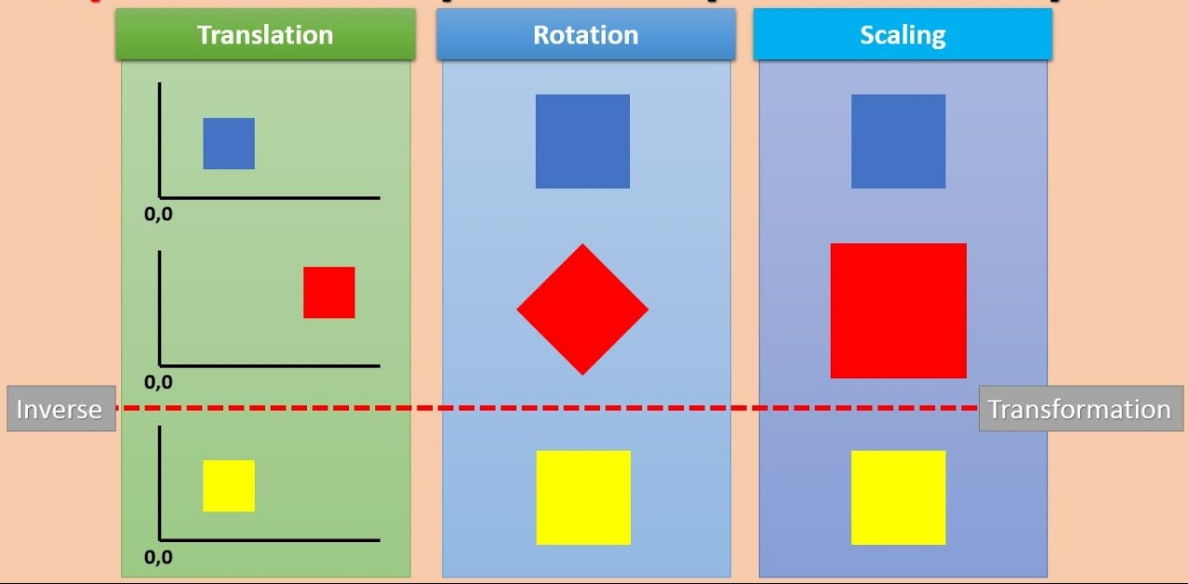
\includegraphics[width=0.8\textwidth]{2022_TallerGraficacion/Figs/Transformaciones2D}
 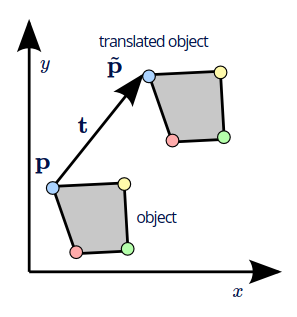
\includegraphics[width=0.45\textwidth]{2022_TallerGraficacion/Figs/Traslacion}
     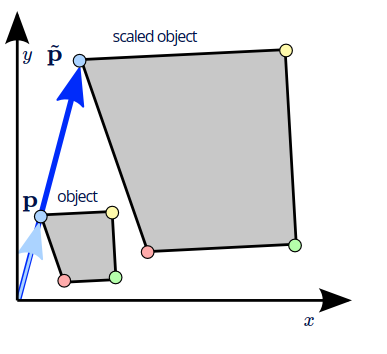
\includegraphics[width=0.52\textwidth]{2022_TallerGraficacion/Figs/Escalamiento}\\
  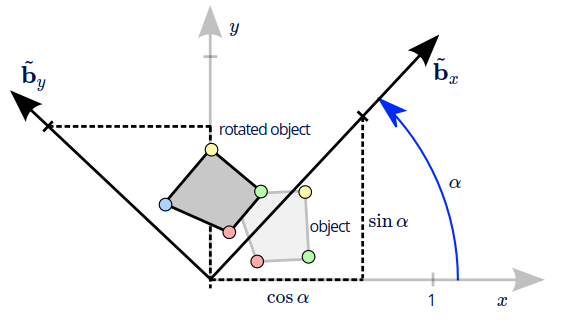
\includegraphics[width=0.7\textwidth]{2022_TallerGraficacion/Figs/Rotacion}

 \end{center}
\end{column}
\end{columns}

\end{frame}



\begin{frame}{Dibujar una esfera (1)}
\begin{columns}
\begin{column}{0.5\textwidth}
\begin{itemize}
\item La definición de esfera es una superficie cerrada en 3D donde cada punto de la esfera está a la misma distancia (radio) de un punto dado.
\item Dado que no podemos dibujar todos los puntos en una esfera, solo tomamos muestras de una cantidad limitada de puntos dividiendo la esfera por sectores (longitud) y pilas (latitud).
\end{itemize}

\end{column}
\begin{column}{0.5\textwidth}
\begin{center}
 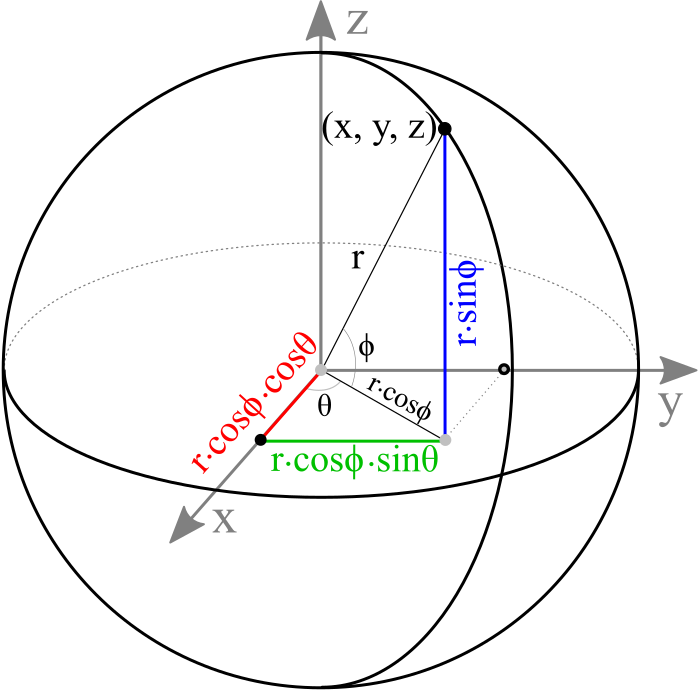
\includegraphics[width=0.8\textwidth]{2022_TallerGraficacion/Figs/gl_sphere01}
 \end{center}
\end{column}
\end{columns}
\footnotetext{\url{http://www.songho.ca/opengl/gl_sphere.html}}


\end{frame}

\begin{frame}{Dibujar una esfera (2)}
\begin{columns}
\begin{column}{0.4\textwidth}
\begin{itemize}
\item Para dibujar la superficie de una esfera en OpenGL, debe triangular los vértices adyacentes para formar polígonos. Es posible usar una sola tira triangular para renderizar toda la esfera.
\item Cada sector de una pila requiere 2 triángulos.
\end{itemize}
\begin{block}{Demo \#4}
Esfera en OpenGL ES
\end{block}

\end{column}
\begin{column}{0.3\textwidth}
\begin{center}
 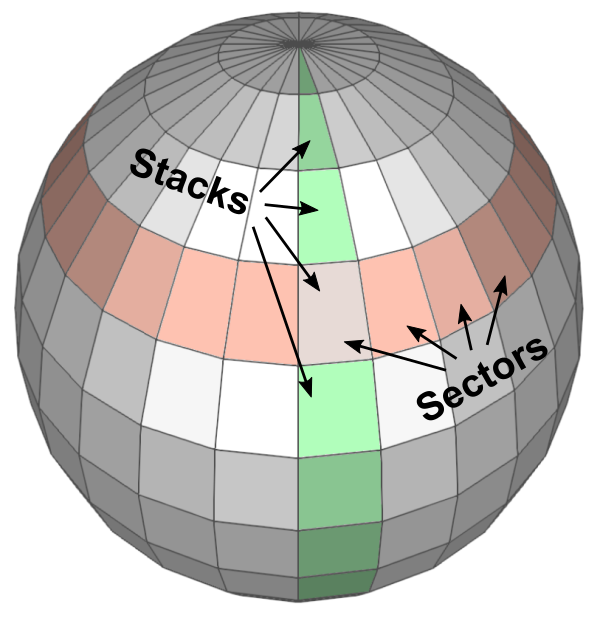
\includegraphics[width=0.98\textwidth]{2022_TallerGraficacion/Figs/gl_sphere02}
 \end{center}

\end{column}
\begin{column}{0.3\textwidth}
\begin{center}
 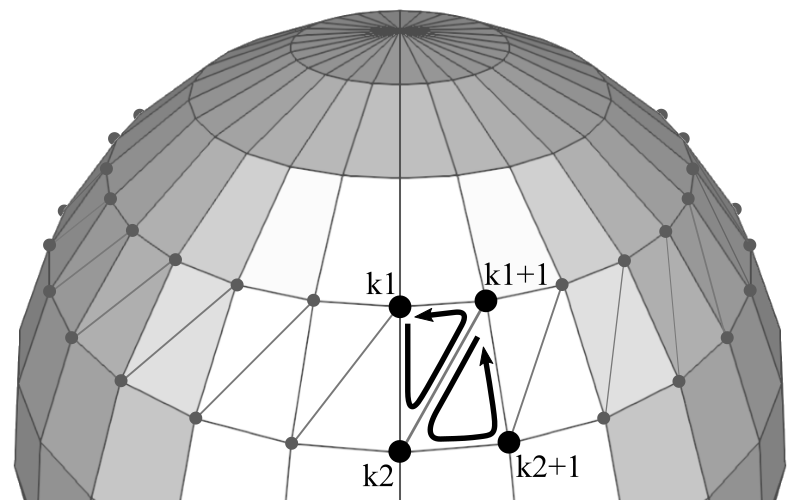
\includegraphics[width=0.98\textwidth]{2022_TallerGraficacion/Figs/gl_sphere03}
 \end{center}
\end{column}
\end{columns}


\end{frame}


%\section{Texturas}
\begin{frame}{Mapeo de Texturas}
%\begin{block}{Demo \#5}
%Texturas en OpenGL
%\end{block}
\begin{columns}
\begin{column}{0.6\textwidth}
\begin{itemize}
\item El mapeo de texturas en gráficos por computadora se refiere a la aplicación de un tipo de superficie a una imagen 3D. 
%\item Una textura puede ser uniforme, como una pared de ladrillos, o irregular, como vetas de madera o mármol. 
\item El método común es crear una imagen de mapa de bits 2D de la textura, llamada \textit{mapa de textura}, que luego se \textit{envuelve} alrededor del objeto 3D. 
\item Para texturas mas precisas se emplean funciones matemáticas en lugar de mapas de bits.
\end{itemize}
\begin{block}{Demo \#5}
Texturas en OpenGL
\end{block}
\end{column}
\begin{column}{0.4\textwidth}
    \begin{center}
         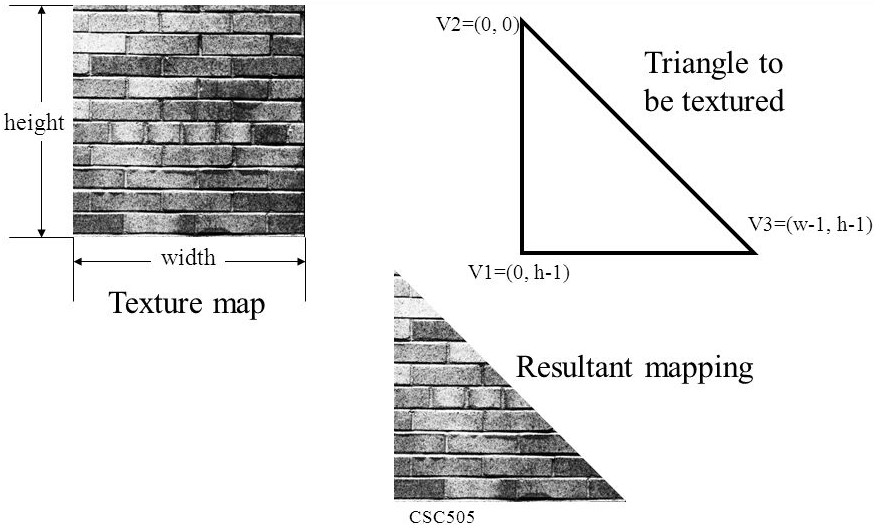
\includegraphics[width=0.98\textwidth]{2022_TallerGraficacion/Figs/Textures}
     \end{center}
\end{column}
\end{columns}
\end{frame}

\begin{frame}{Multiples Texturas en OpenGL}
%\begin{block}{Demo \#6}
%Multiples Texturas en OpenGL
%\end{block}
\begin{columns}
\begin{column}{0.5\textwidth}
\begin{itemize}
\item 
\end{itemize}
    \begin{center}
        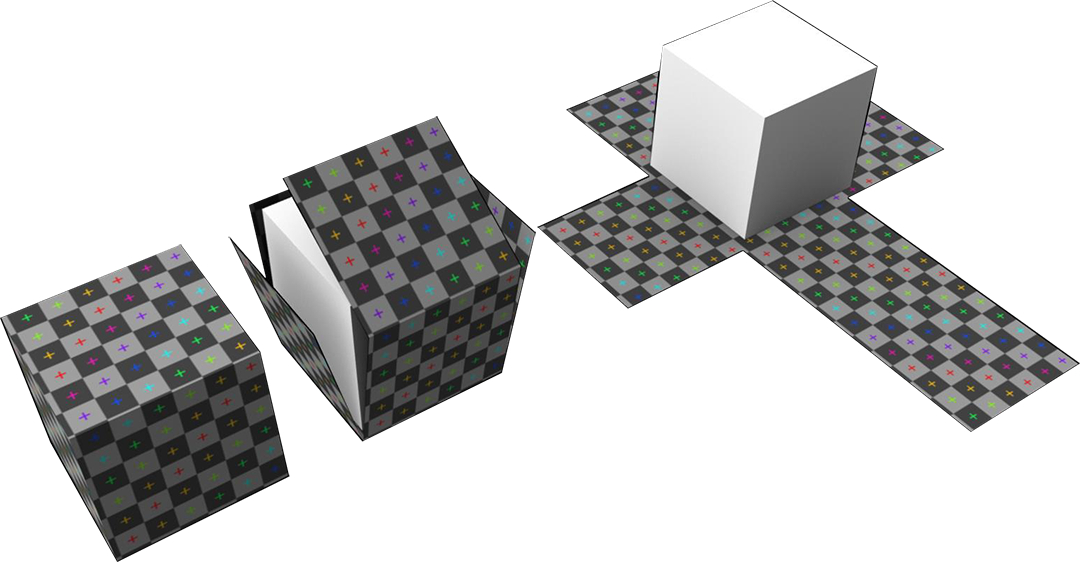
\includegraphics[width=0.98\textwidth]{2022_TallerGraficacion/Figs/RefImgBoxmap2}
     \end{center}
\begin{block}{Demo \#6}
Multiples Texturas en OpenGL
\end{block}
\end{column}
\begin{column}{0.5\textwidth}
    \begin{center}
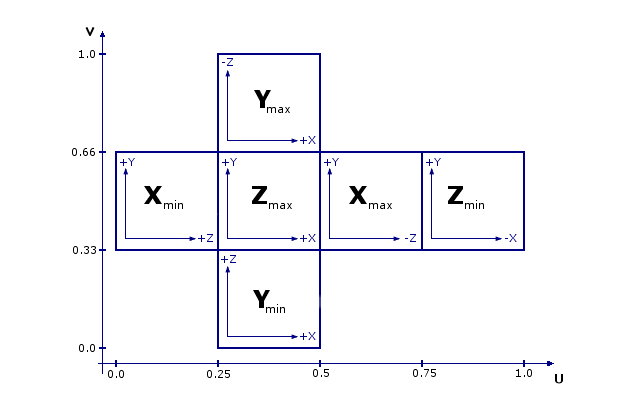
\includegraphics[width=0.98\textwidth]{2022_TallerGraficacion/Figs/RefImgBoxmap}
%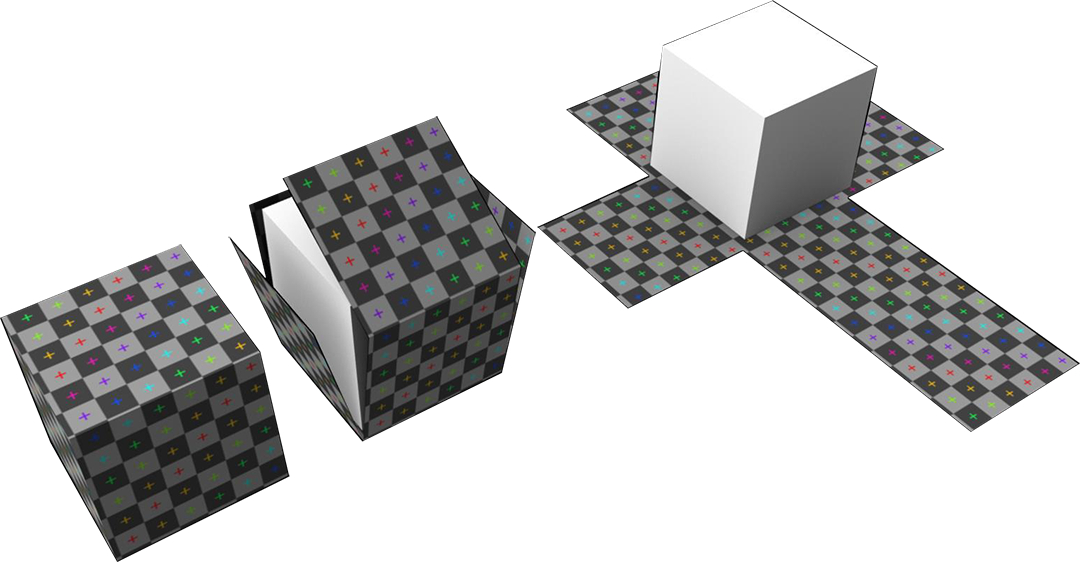
\includegraphics[width=0.98\textwidth]{2022_TallerGraficacion/Figs/RefImgBoxmap2}
     \end{center}
\end{column}
\end{columns}

\end{frame}

\begin{frame}{UV mapping}
\begin{columns}
\begin{column}{0.5\textwidth}
\begin{itemize}
\item El mapeo UV es el proceso de modelado 3D de proyectar una imagen 2D en la superficie de un modelo 3D para el mapeo de texturas. Las letras $U$ y $V$ denotan los ejes de la textura 2D porque $X$, $Y$ y $Z$ ya se utilizan para denotar los ejes del objeto 3D en el espacio modelo,
\end{itemize}
\begin{block}{Demo \#7}
Textura sobre una Esfera
\end{block}
\end{column}
\begin{column}{0.5\textwidth}
    \begin{center}
         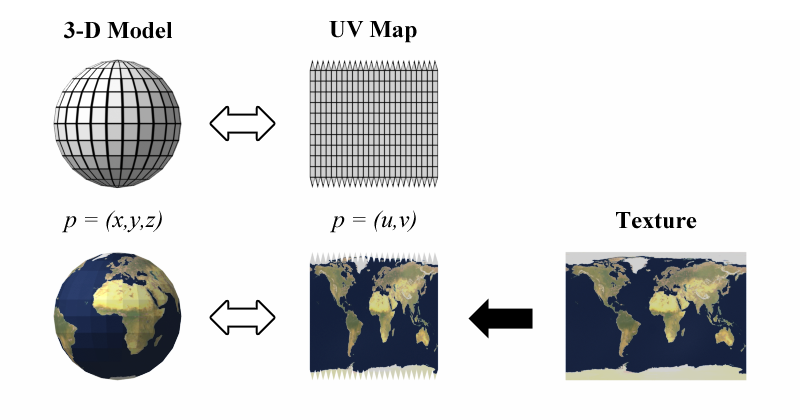
\includegraphics[width=0.98\textwidth]{2022_TallerGraficacion/Figs/UVMapping}
     \end{center}
\end{column}
\end{columns}
\end{frame}



\section{Iluminación y Sombreado}
\begin{frame}{Iluminación Ambiente y Difusa}
\begin{columns}
\begin{column}{0.5\textwidth}
\begin{itemize}
\item Iluminación ambiental: lo que los objetos nunca están completamente oscuros. 
\item Iluminación difusa: simula el impacto direccional que tiene un objeto ligero sobre un objeto. 
\item Iluminación especular: simula el punto brillante (del color de la fuente) de una luz que aparece sobre objetos brillantes.
\end{itemize}
\end{column}
\begin{column}{0.5\textwidth}
\begin{center}
 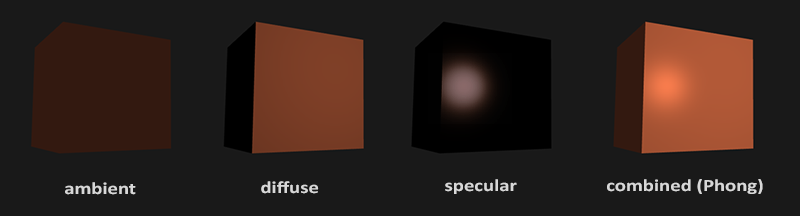
\includegraphics[width=0.98\textwidth]{2022_TallerGraficacion/Figs/basic_lighting_phong}\\
 
\includegraphics[width=0.48\textwidth]{2022_TallerGraficacion/Figs/diffuse_light}
 \end{center}
\end{column}
\end{columns}
\begin{block}{Demo \#8}
Iluminacion Ambiente y Difusa
\end{block}
\end{frame}


%\section{Iluminación y Sombreado}
\begin{frame}{Iluminación por Vertices}
\begin{columns}
\begin{column}{0.5\textwidth}
\begin{itemize}
\item En la iluminación por vértice, la cara frontal del cubo muestra un sombreada plana sin evidencia de indicencia de luz. Los cuatro puntos de la cara frontal son equidistantes de la luz, y intensidad en cada puntos es interpolada mediante los triángulos que forman la cara frontal.
\item En la iluminación por fragmento hay un efecto mucho más notorio en la misma cara del cubo.
\end{itemize}
\begin{block}{Demo \#9}
Iluminación por Fragmentos
\end{block}

\end{column}
\begin{column}{0.5\textwidth}
\begin{center}
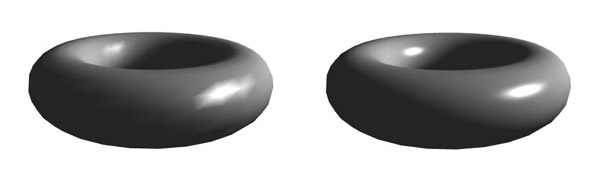
\includegraphics[width=0.48\textwidth]{2022_TallerGraficacion/Figs/specular3}\\
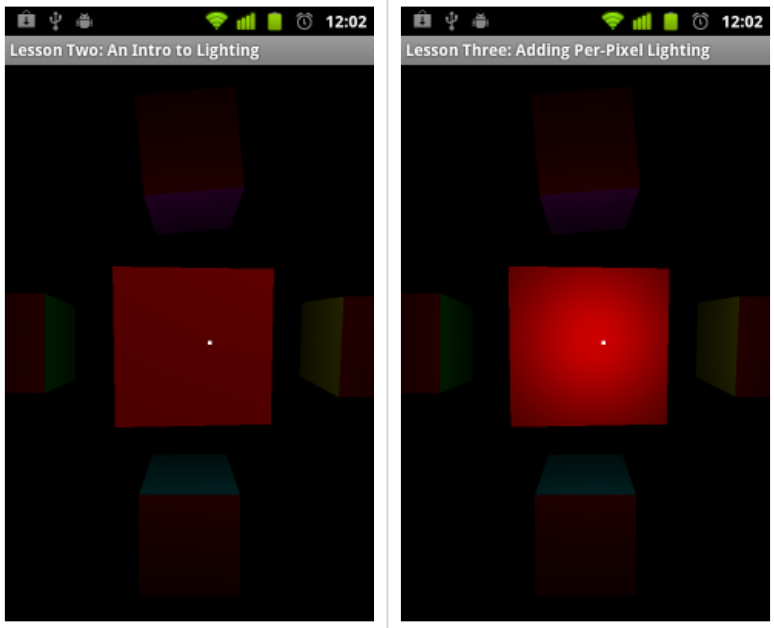
\includegraphics[width=0.78\textwidth]{2022_TallerGraficacion/Figs/PerPixelVsPerFragmentShading}
 \end{center}
\end{column}
\end{columns}

\end{frame}



\begin{frame}{Textura e Iluminación}
\begin{columns}
\begin{column}{0.5\textwidth}
\begin{itemize}
\item El arte del mapeo de texturas (junto con la iluminación) es relevabnte para construir ambientes 3D de apariencia realista. Sin esto, el sombreado suavemente parecerá artificial, como un viejo juego de consola de los años 90.
\item Para lograr esto, es necesario enviar al vertex shader una matriz con información de coordenadas de textura. 
\end{itemize}
\begin{block}{Demo \#10}
Textura e Iluminación
\end{block}
\end{column}
\begin{column}{0.5\textwidth}
\begin{center}
% 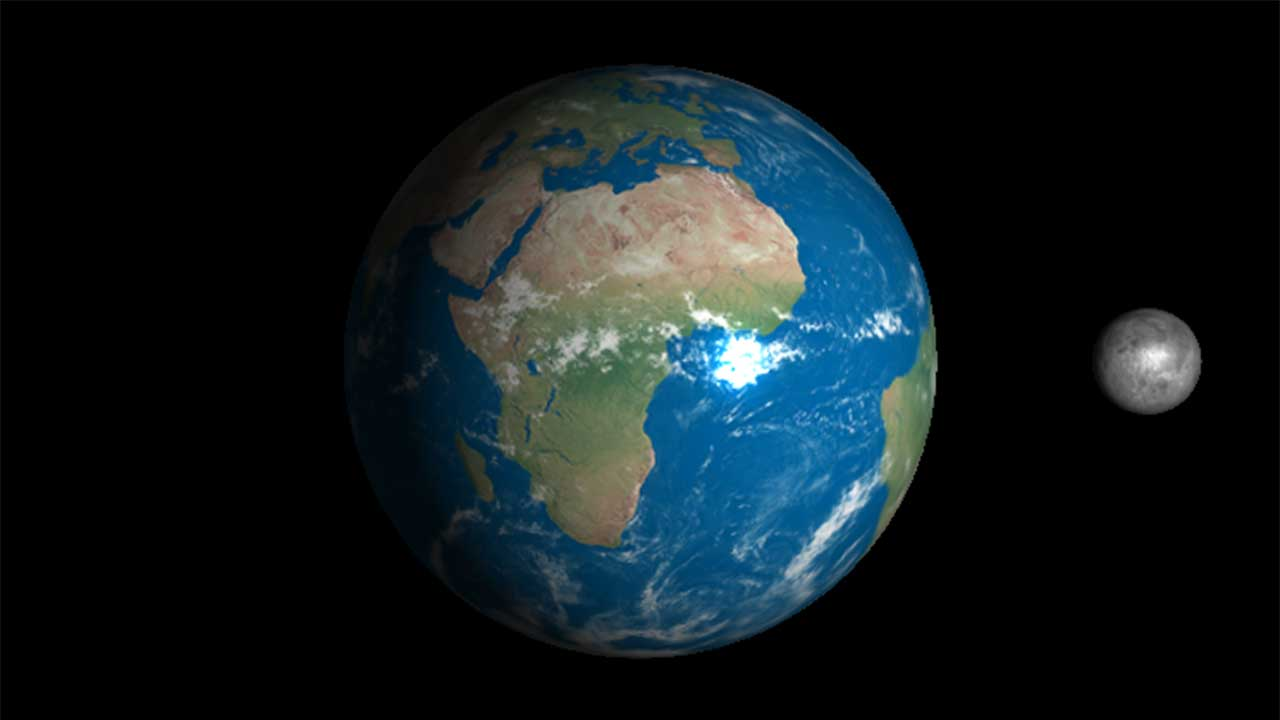
\includegraphics[width=0.98\textwidth]{2022_TallerGraficacion/Figs/OpenGL_TexturingAndLighting}
 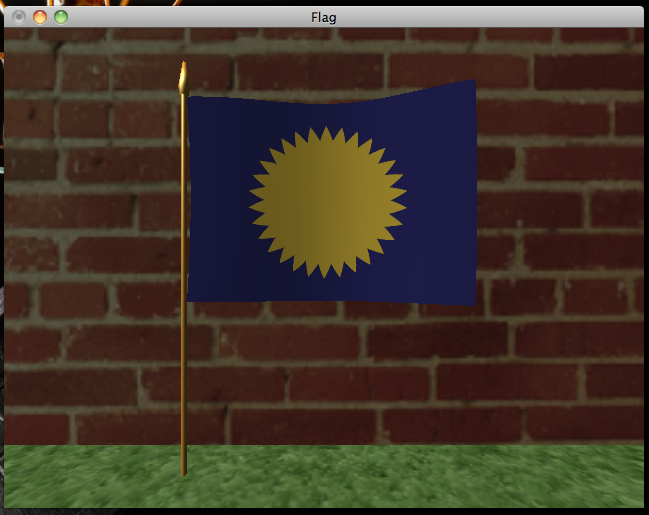
\includegraphics[width=0.98\textwidth]{2022_TallerGraficacion/Figs/Textura_e_Iluminacion}
\end{center}
\end{column}
\end{columns}

\end{frame}

\begin{frame}{Textura e Iluminación Sobre una Esfera}
\begin{columns}
\begin{column}{0.5\textwidth}
\begin{itemize}
\item Para agregar realismo a las escenas, es necesario combinar texturas más iluminación.
\item El código en el \textit{Fragment Shader} es más complejo para lograr dicha tarea. 
\end{itemize}
\begin{block}{Demo \#11}
Textura e Iluminación sobre una Esfera
\end{block}
\end{column}
\begin{column}{0.5\textwidth}
\begin{center}
 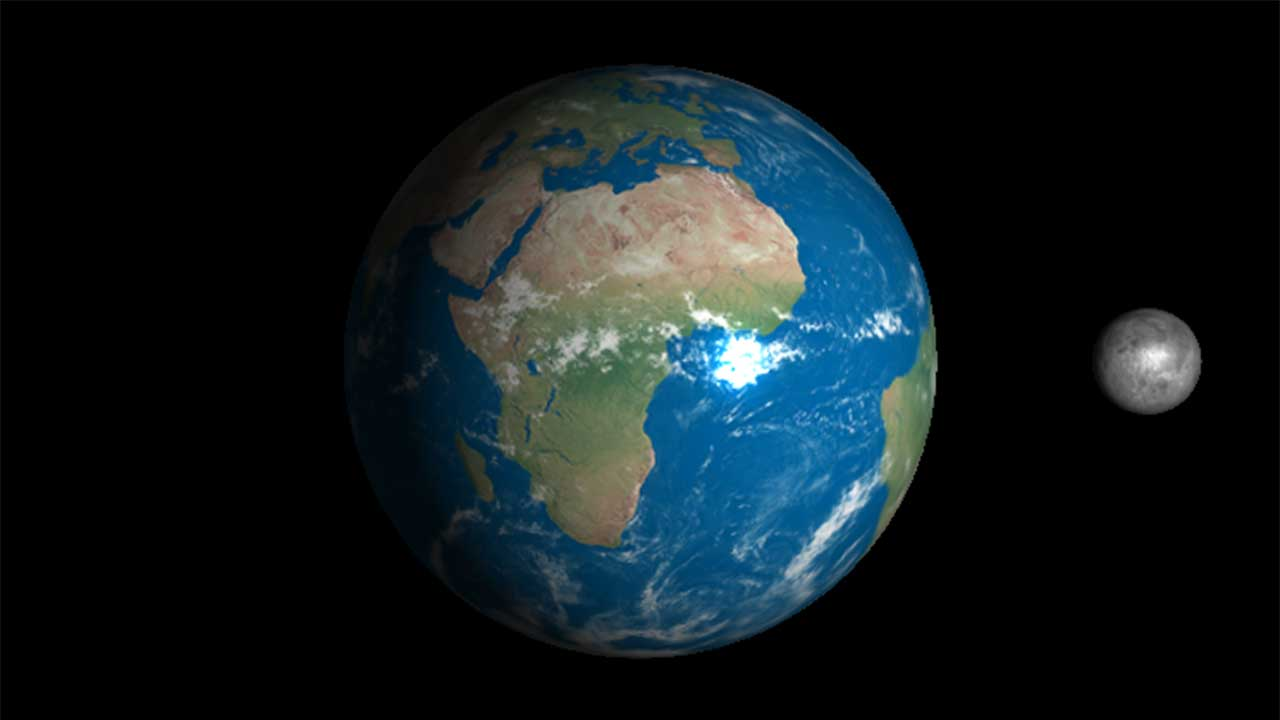
\includegraphics[width=0.98\textwidth]{2022_TallerGraficacion/Figs/OpenGL_TexturingAndLighting}
% 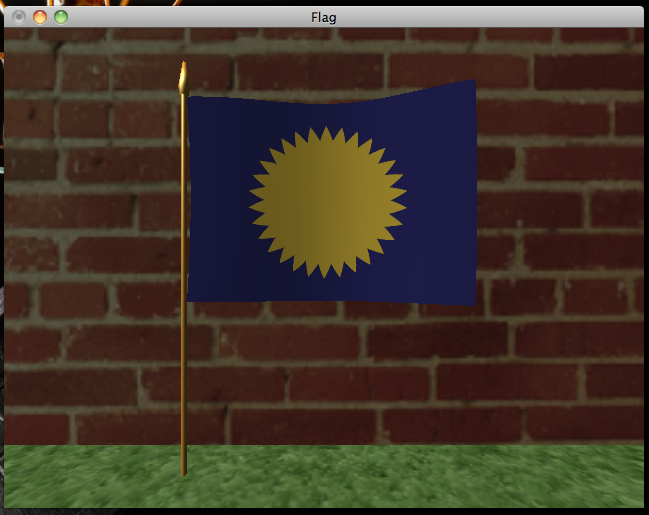
\includegraphics[width=0.98\textwidth]{2022_TallerGraficacion/Figs/Textura_e_Iluminacion}
\end{center}
\end{column}
\end{columns}

\end{frame}

%\begin{frame}{}
%\begin{block}{Demo \#12}
%Globo
%\end{block}
%\end{frame}




%\section{Tópicos Avanzados}
%\begin{frame}{Vertex Buffer Objects (VBO)}
%\begin{itemize}
%  \item Para objetos simples, los datos de objetos en la memoria del lado del cliente están almacenados del lado del cliente, y solo se transfieren a GPU en el momento del renderizado.
%\item A medida que la escenas se vuelve más compleja con más objetos y triángulos, esto puede imponer un costo adicional en el uso de la CPU y la memoria. 
%\item Solución: Vertex Buffer.  En lugar de transferir información de vértices desde la memoria del cliente en cada frame, la información se transferirá una vez y luego se realizará la renderización desde la memoria caché del GPU.
%\end{itemize}
%\begin{block}{Demo \#13}
%Vertex Buffer Object
%\end{block}
%\end{frame}
%\begin{frame}{Index Buffer Objects (IBO) - I}
%\begin{itemize}
%\item La desventaja de los búferes de vértices se produce cuando usamos muchos de los mismos vértices una y otra vez.
%\item Por ejemplo, un mapa de alturas se puede dividir en una serie de tiras triangulares. Dado que cada franja vecina comparte una fila de vértices, terminaremos repitiendo muchos vértices con un búfer de vértices.
%\end{itemize}
%\begin{center}
 %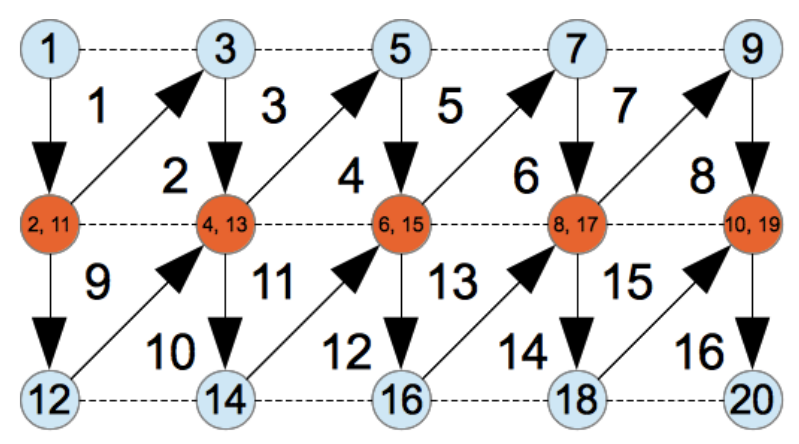
\includegraphics[width=0.5\textwidth]{2022_TallerGraficacion/Figs/IBO_01}
% \end{center}

%\end{frame}

%\begin{frame}{Index Buffer Objects (IBO) - II}
%\begin{columns}
%\begin{column}{0.5\textwidth}
%\begin{itemize}
%\item Podemos usar un objeto de búfer de índice. En lugar de repetir vértices en el búfer de vértices, definiremos cada vértice una vez, y solo una vez. Nos referiremos a estos vértices usando conjuntos o en este búfer de vértices, y cuando necesitemos reutilizar un vértice, repetiremos el conjunto o en lugar de repetir todo el vértice
%\end{itemize}
%\end{column}
%\begin{column}{0.5\textwidth}
%\begin{center}
% 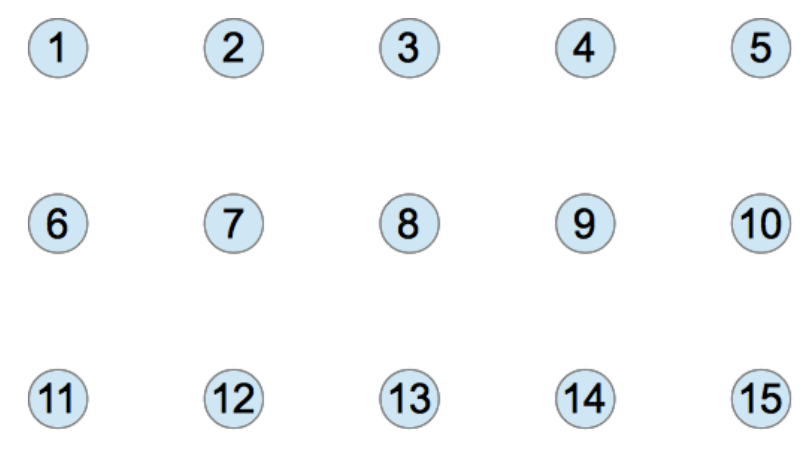
\includegraphics[width=0.95\textwidth]{2022_TallerGraficacion/Figs/IBO_02}
% \end{center}
%\begin{block}{Demo \#14}
%Index Buffer Objects
%\end{block}
%\end{column}
%\end{columns}
%\end{frame}


\begin{frame}{Simulación de Particulas}
\begin{itemize}
\item Una partícula es un diminuto objeto 2D que siempre está frente a la cámara y que generalmente contiene una textura con partes transparentes. 
\item Una partícula en sí misma es efectivamente solo un sprite (mapa de bits), que al combinarse con otros crear efectos asombrosos.
\item Existe un objeto llamado emisor o generador de partículas que, desde su ubicación, genera continuamente nuevas partículas que se descomponen con el tiempo. 
\item Si un emisor de partículas de este tipo generara, por ejemplo, partículas diminutas con una textura similar al humo, las coloreara menos brillantes cuanto mayor sea la distancia del emisor y les diera una apariencia brillante, obtendría un efecto similar al del fuego. 
\end{itemize}
\begin{block}{Demo \#15}
Particulas
\end{block}
\end{frame}

\begin{frame}{Skybox}
\begin{itemize}
\item Imagina que hay una montaña en la distancia dentro de un juego. Una montaña a la que el jugador nunca podrá viajar, porque está muy lejos. 
\item Modelar la geometría real de esa montaña y luego renderizarla en un rango de ángulos realmente estrecho todo el tiempo requeriría recursos de la GPU. 
\item Es mucho más eficiente y bastante efectivo tener solo una imagen renderizada previamente de esa montaña para mostrar. 
\item Un Skybox es caja grande con textura alrededor del mundo para mostrar objetos muy distantes que no se pueden alcanzar.
\end{itemize}

\begin{block}{Demo \#16}
SkyBox
\end{block}
\end{frame}	

%\section{Conclusiones}
%\begin{frame}{Conclusiones}
%\begin{itemize}
%\item En años recientes, se han explorado aplicaciones gráficas en teléfonos inteligentes.
%\item Los teléfonos inteligentes proveen de capacidades de cómputo cada vez mayores.
%\item Las librerías gráficas han tenido una evoluación marcada por la demanda del mercado.
%\item La necesidad de profesionales calificados en mayor. 
%\end{itemize}
%\end{frame}	

